\section{Diseño Orientado a Objetos}
En esta sección, se describen las dos etapas principales del Diseño Orientado a Objetos bajo la metodología OMT++ . Cada etapa del diseño se construye a partir de los resultados obtenidos en etapas anteriores, como el Análisis Orientado a Objetos (AOO) o las especificaciones iniciales del sistema. El propósito de estas etapas es transformar el modelo conceptual en un diseño detallado que pueda ser implementado en un lenguaje de programación, asegurando que las clases y métodos definidos cumplan con los requisitos funcionales y no funcionales del sistema.
El diseño de objetos consiste en establecer los elementos estructurales del sistema, mientras que el diseño del comportamiento se centra en definir cómo interactúan estos elementos para realizar las operaciones del sistema.

 \subsection{Diseño de Objetos}
 En esta etapa, se define la estructura del sistema a partir de los conceptos identificados durante el análisis. Se crea un modelo de objetos del diseño que incluye:

 Las clases del sistema y sus atributos.
 Los métodos necesarios para cumplir con las operaciones.
 La relación entre las clases, aplicando patrones de arquitectura como MVC para organizar la solución en capas (Modelo, Vista y Controlador).
 El diseño de objetos garantiza una organización clara y modular, facilitando la reutilización de componentes y la mantenibilidad del sistema.

 \begin{figure}[H]
	\centering
	\caption{Diagrama Model-View-Controller}
	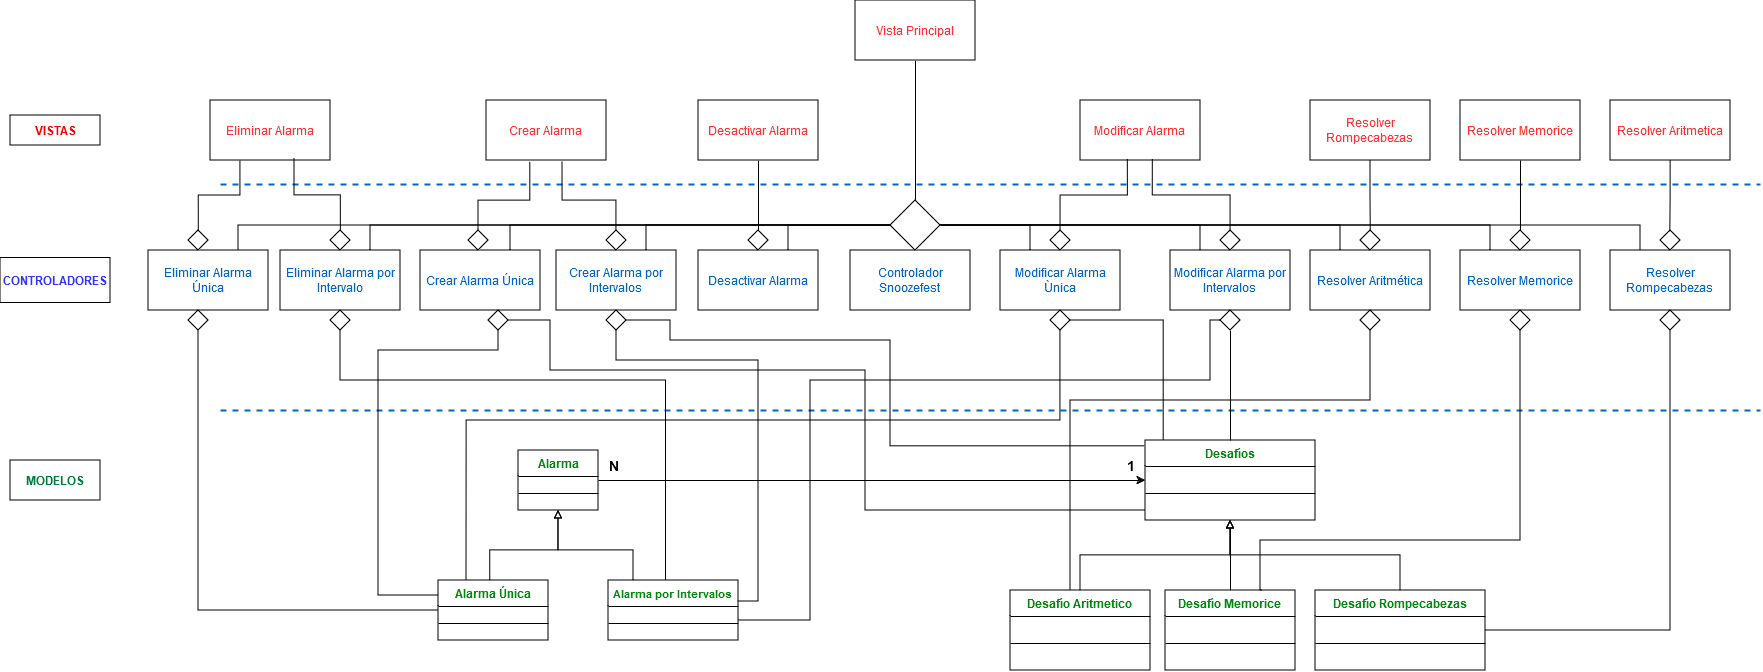
\includegraphics[width=\textwidth]{./img/MVC.png}
        \vspace{10pt}
	\label{fig:Diagrama Model-View-Controller}
\end{figure}

 \subsection{Diseño del Comportamiento}
 Esta etapa complementa el diseño estructural definiendo la interacción entre las clases para cumplir con las operaciones especificadas en el análisis. Utiliza herramientas como:
 
\begin{itemize}
        \item \textbf{Trazas de eventos:} Representan cómo se comunican los objetos del sistema en respuesta a eventos.
        \item \textbf{Diagramas de secuencia (UML):} modelan las interacciones en un flujo temporal, especificando mensajes, llamadas a métodos y valores retornados.
\end{itemize}

El diseño del comportamiento asegura que cada operación del sistema esté respaldada por una secuencia de acciones coherente y eficiente, respetando las responsabilidades asignadas a cada clase. Esto garantiza que el sistema funcione de acuerdo con los requisitos y sea adaptable a cambios futuros.
